%%%%%%%%%%%%%%%%%%%%%%%%%%%%%%%%%%%%%%%%%
% Beamer Presentation
% LaTeX Template
% Version 1.0 (10/11/12)
%
% This template has been downloaded from:
% http://www.LaTeXTemplates.com
%
% License:
% CC BY-NC-SA 3.0 (http://creativecommons.org/licenses/by-nc-sa/3.0/)
%
%%%%%%%%%%%%%%%%%%%%%%%%%%%%%%%%%%%%%%%%%

%----------------------------------------------------------------------------------------
%	PACKAGES AND THEMES
%----------------------------------------------------------------------------------------

\documentclass[9pt, t]{beamer}
\usetheme[progressbar=frametitle]{metropolis}
\metroset{block=fill}

%% Packages
\usepackage{multicol}
\usepackage[english]{babel}
\usepackage{eurosym}
\usepackage{pgfpages}
\usepackage[utf8]{inputenc}
\usepackage[T1]{fontenc}
\usepackage{hyperref}
\usepackage{alltt}
\usepackage{color}
\usepackage{amsmath,amsfonts,amssymb,amsthm}
%\usepackage[ruled,vlined]{algorithm2e}
\usepackage{xspace}
\usepackage[normalem]{ulem}
\usepackage{filemod}
%\usepackage{bibentry}
\usepackage{multicol}
\usepackage[absolute,overlay]{textpos}
\usepackage{array}
\newcounter{chapter} 
\usepackage[framemethod=TikZ]{mdframed}
\usepackage[backend=biber]{biblatex}
\addbibresource{bib.bib}
\usepackage{csquotes}
\usepackage{animate}
\usepackage{caption}
\usepackage{subcaption}
\usepackage{algorithm}
\usepackage[noend]{algpseudocode}
\usepackage{listings}

\usepackage{graphicx} % Allows including images
\usepackage{booktabs} % Allows the use of \toprule, \midrule and \bottomrule in tables

\graphicspath{{assets/}}

%----------------------------------------------------------------------------------------
%	TITLE PAGE
%----------------------------------------------------------------------------------------

\title[Signal Image \& Video]{Skeletonization of Binary Images} % The short title appears at the bottom of every slide, the full title is only on the title page

\author{Filippo Momesso} % Your name
\institute[UniTN] % Your institution as it will appear on the bottom of every slide, may be shorthand to save space
{
University of Trento \\ % Your institution for the title page
\medskip
\textit{filippo.momesso@studenti.unitn.it} % Your email address
}
\date{\today} % Date, can be changed to a custom date

\begin{document}

\begin{frame}
  \titlepage % Print the title page as the first slide
\end{frame}

\begin{frame}
  \frametitle{Overview} % Table of contents slide, comment this block out to remove it
  \tableofcontents % Throughout your presentation, if you choose to use \section{} and \subsection{} commands, these will automatically be printed on this slide as an overview of your presentation
\end{frame}

%------------------------------------------------------------------
%	PRESENTATION SLIDES
%------------------------------------------------------------------
\section{Basic definitions}
\begin{frame}
  \frametitle{What is Skeletonization?}
  \begin{block}{Skeletonization}
    An image processing technique which reduces a binary object (or region) to a 1 pixel wide representation called \textbf{skeleton}.
  \end{block}
  Useful in many application fields such as \emph{shape recognition and analysis}, \emph{animation}, \emph{motion tracking} or \emph{medical imaging}~\cite{skel-applications}.
  \begin{figure}
    \begin{center}
      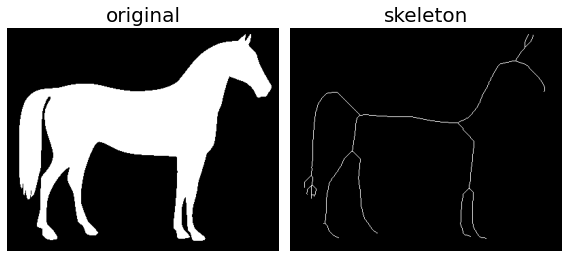
\includegraphics[width=0.6\textwidth]{skeletonization-example.png}
      \caption{Example of a skeletonized image.}
    \end{center}
  \end{figure}
\end{frame}

\begin{frame}
  \label{sli:skeleton}
  \frametitle{What is Skeletonization?}
  \begin{block}{Skeleton}
    The ideal skeleton should:
    \begin{itemize}
      \item be a \textbf{connected subset} of points from the original region,
      \item represent the \textbf{geometric} characteristics of the region,
      \item preserve the \textbf{topological} characteristics of the region (e.g. connectivity, holes, cavities...)
    \end{itemize}
  \end{block}

  Three major skeletonization techniques:
  \begin{itemize}
    \item Medial-axis distance transform
    \item Non-pixel-based methods (computes analytically the skeleton)
    \item Thinning methods.
  \end{itemize}
  \vspace{0.5cm}
  We will focus on \textbf{thinning methods} since they are quite efficient and commonly used in state-of-the-art applications.
\end{frame}

\section{Zhang-Suen Parallalel Thinning}
\begin{frame}
  \frametitle{Zhang-Suen Parallalel Thinning}
  \textbf{Zhang-Suen algorithm}~\cite{zha84} is a fast parallel algorithm which takes a binary 2D image and removes pixels from the object's border by making successive iterations until convergence.
  \begin{block}{2D Binary image}
    A matrix $M$ where each pixel $M[i][j]$ is either $1$ or $0$. A \textbf{region} in an image is a connected set of $1$-valued pixels.
  \end{block}
  \begin{columns}
    \begin{column}{0.5\textwidth}
      \begin{figure}
        \centering
        
\includegraphics[width=0.5\textwidth]{region-example.png}
        \caption{In white a region.}
      \end{figure}
    \end{column}
    \begin{column}{0.5\textwidth}
      \begin{figure}
        \centering
        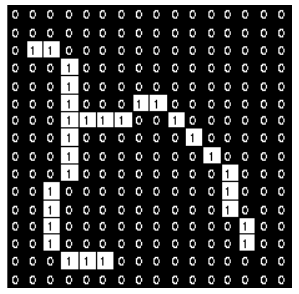
\includegraphics[width=0.5\textwidth]{skel-region-example.png}
        \caption{The skeleton of the region on the left.}
      \end{figure}
    \end{column}
  \end{columns}
\end{frame}

\begin{frame}
  \frametitle{Zhang-Suen Parallalel Thinning}
  \begin{itemize}
    \item Given an element $P_1 = M[i][j]$, its neighbours are:
          \begin{center}
            \setlength{\arrayrulewidth}{0.3mm}
            \renewcommand{\arraystretch}{2}
            \begin{tabular}{|c|c|c|}
              \hline
              $P_9 = M[i-1][j-1]$ & $P_2 = M[i-1][j]$ & $P_3 = M[i-1][j+1]$ \\
              \hline
              $P_8 = M[i][j-1]$   & $P_1 = M[i][j]$   & $P_4 = M[i][j+1]$   \\
              \hline
              $P_7 = M[i+1][j-1]$ & $P_6 = M[i+1][j]$ & $P_5 = M[i+1][j+1]$ \\
              \hline
            \end{tabular}
          \end{center}

          \vspace{0.5cm}
    \item The algorithm iteratively removes all countour points (change the value from 1 to 0) which satisfy some conditions on their 8 neighbours.
          \\~\\
    \item The new value of a pixel at the $n$-th iteration is based on the values of its neighbours at the $n-1$-th iteration. This allows all pixel to be processed in \textbf{parallel} in each iteration.
  \end{itemize}
\end{frame}

\begin{frame}
  \frametitle{Pixel Deletion Conditions}
  \begin{itemize}
    \item An iteration (full pass over all the pixels) is divided in two sub-iterations.
          \\~\\
    \item \textbf{Sub-iteration 1}: $P_1$ is deleted if
          \begin{enumerate}
            \item $2 \leq B(P_1) \leq 6$
            \item $A(P_1) = 1$
            \item $P_2 * P_4 * P_6 = 0$
            \item $P_4 * P_6 * P_8 = 0$
          \end{enumerate}
          \vspace{0.3cm}
    \item \textbf{Sub-iteration 2}: $P_1$ is deleted if
          \begin{enumerate}
            \item Conditions 1 and 2 are true
            \item $P_2 * P_4 * P_8 = 0$
            \item $P_2 * P_6 * P_8 = 0$
          \end{enumerate}
          \vspace{0.3cm}
    \item $B(P_1)$ is the number of \textbf{1-value neighbours} of $P_1$. Condition 1 is needed to textbf{preserve an endpoint} of the skeleton.
    \item $A(P_1)$ is the number of \textbf{0-1 patterns} in the ordered sequence of neighbours $P_2, P_3, \dots, P_9, P_2$. Condition 2 is needed to preserve \textbf{connectivity}, i.e. not split the skeleton in two.
  \end{itemize}
\end{frame}

\begin{frame}
  \frametitle{Pixel Deletion Conditions}
  \begin{figure}
    \centering
    \begin{subfigure}[b]{0.3\textwidth}
      \centering
      
\includegraphics[width=\textwidth]{simple-zhang/img_000.png}
      \caption{Original image.}
    \end{subfigure}
    \hfill
    \begin{subfigure}[b]{0.3\textwidth}
      \centering
      
\includegraphics[width=\textwidth]{simple-zhang/img_011.png}
      \caption{After sub-iteration 1.}
    \end{subfigure}
    \hfill
    \begin{subfigure}[b]{0.3\textwidth}
      \centering
      
\includegraphics[width=\textwidth]{simple-zhang/img_014.png}
      \caption{After sub-iteration 2.}
    \end{subfigure}
    \caption{Effects of one single iteration on an example image.}
  \end{figure}
  Thanks to conditions 3 and 4:
  \begin{itemize}
    \item Sub-iteration 1 removes East and South boundary pixels and North-West corner pixels.
    \item Sub-iteration 2 removes West and North boundary pixels and South-East corner pixels.
  \end{itemize}
\end{frame}

\begin{frame}[c]
  \frametitle{Zhang-Suen Visualization}
  \centering
  \begin{figure}
  \animategraphics[loop, autoplay,width=0.5\textwidth]{15}{../zhang/img_}{000}{047}
  \caption{Animation of Zhang-Suen algorithm removing contour pixels until only the skeleton remains.}
  \end{figure}
\end{frame}

\begin{frame}
  \frametitle{Zhang-Suen Pseudocode}
  \section{Zhang-Suen Parallalel Thinning}
\begin{frame}
  \frametitle{Zhang-Suen Parallalel Thinning}
  \textbf{Zhang-Suen algorithm}~\cite{zha84} is a fast parallel algorithm which takes a binary 2D image and removes pixels from the object's border by making successive iterations until convergence.
  \begin{block}{2D Binary image}
    A matrix $M$ where each pixel $M[i][j]$ is either $1$ or $0$. A \textbf{region} in an image is a connected set of $1$-valued pixels.
  \end{block}
  \begin{columns}
    \begin{column}{0.5\textwidth}
      \begin{figure}
        \centering
        
\includegraphics[width=0.5\textwidth]{region-example.png}
        \caption{In white a region.}
      \end{figure}
    \end{column}
    \begin{column}{0.5\textwidth}
      \begin{figure}
        \centering
        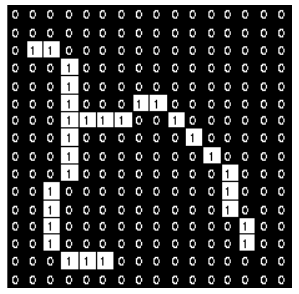
\includegraphics[width=0.5\textwidth]{skel-region-example.png}
        \caption{The skeleton of the region on the left.}
      \end{figure}
    \end{column}
  \end{columns}
\end{frame}

\begin{frame}
  \frametitle{Zhang-Suen Parallalel Thinning}
  \begin{itemize}
    \item Given an element $P_1 = M[i][j]$, its neighbours are:
          \begin{center}
            \setlength{\arrayrulewidth}{0.3mm}
            \renewcommand{\arraystretch}{2}
            \begin{tabular}{|c|c|c|}
              \hline
              $P_9 = M[i-1][j-1]$ & $P_2 = M[i-1][j]$ & $P_3 = M[i-1][j+1]$ \\
              \hline
              $P_8 = M[i][j-1]$   & $P_1 = M[i][j]$   & $P_4 = M[i][j+1]$   \\
              \hline
              $P_7 = M[i+1][j-1]$ & $P_6 = M[i+1][j]$ & $P_5 = M[i+1][j+1]$ \\
              \hline
            \end{tabular}
          \end{center}

          \vspace{0.5cm}
    \item The algorithm iteratively removes all countour points (change the value from 1 to 0) which satisfy some conditions on their 8 neighbours.
          \\~\\
    \item The new value of a pixel at the $n$-th iteration is based on the values of its neighbours at the $n-1$-th iteration. This allows all pixel to be processed in \textbf{parallel} in each iteration.
  \end{itemize}
\end{frame}

\begin{frame}
  \frametitle{Pixel Deletion Conditions}
  \begin{itemize}
    \item An iteration (full pass over all the pixels) is divided in two sub-iterations.
          \\~\\
    \item \textbf{Sub-iteration 1}: $P_1$ is deleted if
          \begin{enumerate}
            \item $2 \leq B(P_1) \leq 6$
            \item $A(P_1) = 1$
            \item $P_2 * P_4 * P_6 = 0$
            \item $P_4 * P_6 * P_8 = 0$
          \end{enumerate}
          \vspace{0.3cm}
    \item \textbf{Sub-iteration 2}: $P_1$ is deleted if
          \begin{enumerate}
            \item Conditions 1 and 2 are true
            \item $P_2 * P_4 * P_8 = 0$
            \item $P_2 * P_6 * P_8 = 0$
          \end{enumerate}
          \vspace{0.3cm}
    \item $B(P_1)$ is the number of \textbf{1-value neighbours} of $P_1$. Condition 1 is needed to textbf{preserve an endpoint} of the skeleton.
    \item $A(P_1)$ is the number of \textbf{0-1 patterns} in the ordered sequence of neighbours $P_2, P_3, \dots, P_9, P_2$. Condition 2 is needed to preserve \textbf{connectivity}, i.e. not split the skeleton in two.
  \end{itemize}
\end{frame}

\begin{frame}
  \frametitle{Pixel Deletion Conditions}
  \begin{figure}
    \centering
    \begin{subfigure}[b]{0.3\textwidth}
      \centering
      
\includegraphics[width=\textwidth]{simple-zhang/img_000.png}
      \caption{Original image.}
    \end{subfigure}
    \hfill
    \begin{subfigure}[b]{0.3\textwidth}
      \centering
      
\includegraphics[width=\textwidth]{simple-zhang/img_011.png}
      \caption{After sub-iteration 1.}
    \end{subfigure}
    \hfill
    \begin{subfigure}[b]{0.3\textwidth}
      \centering
      
\includegraphics[width=\textwidth]{simple-zhang/img_014.png}
      \caption{After sub-iteration 2.}
    \end{subfigure}
    \caption{Effects of one single iteration on an example image.}
  \end{figure}
  Thanks to conditions 3 and 4:
  \begin{itemize}
    \item Sub-iteration 1 removes East and South boundary pixels and North-West corner pixels.
    \item Sub-iteration 2 removes West and North boundary pixels and South-East corner pixels.
  \end{itemize}
\end{frame}

\begin{frame}[c]
  \frametitle{Zhang-Suen Visualization}
  \centering
  \begin{figure}
  \animategraphics[loop, autoplay,width=0.5\textwidth]{15}{../zhang/img_}{000}{047}
  \caption{Animation of Zhang-Suen algorithm removing contour pixels until only the skeleton remains.}
  \end{figure}
\end{frame}

\begin{frame}
  \frametitle{Zhang-Suen Pseudocode}
  \section{Zhang-Suen Parallalel Thinning}
\begin{frame}
  \frametitle{Zhang-Suen Parallalel Thinning}
  \textbf{Zhang-Suen algorithm}~\cite{zha84} is a fast parallel algorithm which takes a binary 2D image and removes pixels from the object's border by making successive iterations until convergence.
  \begin{block}{2D Binary image}
    A matrix $M$ where each pixel $M[i][j]$ is either $1$ or $0$. A \textbf{region} in an image is a connected set of $1$-valued pixels.
  \end{block}
  \begin{columns}
    \begin{column}{0.5\textwidth}
      \begin{figure}
        \centering
        
\includegraphics[width=0.5\textwidth]{region-example.png}
        \caption{In white a region.}
      \end{figure}
    \end{column}
    \begin{column}{0.5\textwidth}
      \begin{figure}
        \centering
        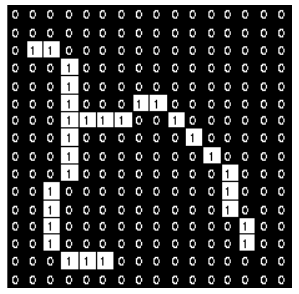
\includegraphics[width=0.5\textwidth]{skel-region-example.png}
        \caption{The skeleton of the region on the left.}
      \end{figure}
    \end{column}
  \end{columns}
\end{frame}

\begin{frame}
  \frametitle{Zhang-Suen Parallalel Thinning}
  \begin{itemize}
    \item Given an element $P_1 = M[i][j]$, its neighbours are:
          \begin{center}
            \setlength{\arrayrulewidth}{0.3mm}
            \renewcommand{\arraystretch}{2}
            \begin{tabular}{|c|c|c|}
              \hline
              $P_9 = M[i-1][j-1]$ & $P_2 = M[i-1][j]$ & $P_3 = M[i-1][j+1]$ \\
              \hline
              $P_8 = M[i][j-1]$   & $P_1 = M[i][j]$   & $P_4 = M[i][j+1]$   \\
              \hline
              $P_7 = M[i+1][j-1]$ & $P_6 = M[i+1][j]$ & $P_5 = M[i+1][j+1]$ \\
              \hline
            \end{tabular}
          \end{center}

          \vspace{0.5cm}
    \item The algorithm iteratively removes all countour points (change the value from 1 to 0) which satisfy some conditions on their 8 neighbours.
          \\~\\
    \item The new value of a pixel at the $n$-th iteration is based on the values of its neighbours at the $n-1$-th iteration. This allows all pixel to be processed in \textbf{parallel} in each iteration.
  \end{itemize}
\end{frame}

\begin{frame}
  \frametitle{Pixel Deletion Conditions}
  \begin{itemize}
    \item An iteration (full pass over all the pixels) is divided in two sub-iterations.
          \\~\\
    \item \textbf{Sub-iteration 1}: $P_1$ is deleted if
          \begin{enumerate}
            \item $2 \leq B(P_1) \leq 6$
            \item $A(P_1) = 1$
            \item $P_2 * P_4 * P_6 = 0$
            \item $P_4 * P_6 * P_8 = 0$
          \end{enumerate}
          \vspace{0.3cm}
    \item \textbf{Sub-iteration 2}: $P_1$ is deleted if
          \begin{enumerate}
            \item Conditions 1 and 2 are true
            \item $P_2 * P_4 * P_8 = 0$
            \item $P_2 * P_6 * P_8 = 0$
          \end{enumerate}
          \vspace{0.3cm}
    \item $B(P_1)$ is the number of \textbf{1-value neighbours} of $P_1$. Condition 1 is needed to textbf{preserve an endpoint} of the skeleton.
    \item $A(P_1)$ is the number of \textbf{0-1 patterns} in the ordered sequence of neighbours $P_2, P_3, \dots, P_9, P_2$. Condition 2 is needed to preserve \textbf{connectivity}, i.e. not split the skeleton in two.
  \end{itemize}
\end{frame}

\begin{frame}
  \frametitle{Pixel Deletion Conditions}
  \begin{figure}
    \centering
    \begin{subfigure}[b]{0.3\textwidth}
      \centering
      
\includegraphics[width=\textwidth]{simple-zhang/img_000.png}
      \caption{Original image.}
    \end{subfigure}
    \hfill
    \begin{subfigure}[b]{0.3\textwidth}
      \centering
      
\includegraphics[width=\textwidth]{simple-zhang/img_011.png}
      \caption{After sub-iteration 1.}
    \end{subfigure}
    \hfill
    \begin{subfigure}[b]{0.3\textwidth}
      \centering
      
\includegraphics[width=\textwidth]{simple-zhang/img_014.png}
      \caption{After sub-iteration 2.}
    \end{subfigure}
    \caption{Effects of one single iteration on an example image.}
  \end{figure}
  Thanks to conditions 3 and 4:
  \begin{itemize}
    \item Sub-iteration 1 removes East and South boundary pixels and North-West corner pixels.
    \item Sub-iteration 2 removes West and North boundary pixels and South-East corner pixels.
  \end{itemize}
\end{frame}

\begin{frame}[c]
  \frametitle{Zhang-Suen Visualization}
  \centering
  \begin{figure}
  \animategraphics[loop, autoplay,width=0.5\textwidth]{15}{../zhang/img_}{000}{047}
  \caption{Animation of Zhang-Suen algorithm removing contour pixels until only the skeleton remains.}
  \end{figure}
\end{frame}

\begin{frame}
  \frametitle{Zhang-Suen Pseudocode}
  \input{assets/pseudocode/zhang.tex}
\end{frame}

\end{frame}

\end{frame}

\section{Morphological Thinning}
\begin{frame}
  \frametitle{Morphological Thinning}
  \textbf{Morphological Thinning}~\cite{morph} is a morphological operation that removes contour pixels from a region of a binary image. It relies on the \textbf{Hit-or-Miss transform} operation.
  \begin{block}
    {Hit-or-Miss transform}
    General binary morphological operation used to look for the presence of specific patterns of \emph{foreground} and \emph{background pixels} (1s or 0s respectively).
  \end{block}
  \begin{columns}
    \begin{column}{0.7\textwidth}
      \begin{itemize}
        \item Hit-or-Miss transform uses a \emph{structuring element} or \emph{kernel} to look for those patterns. \item Tipycally it is used a $3\times3$ kernel. It can contain both 1s and 0s and a special "I don't care" value.
        \item Iteration over all pixels, comparing the kernel with the underlying sub-image.
        \item \lstinline{M[i][j]}$= \begin{cases} 1 & \mbox{if } kernel =$ \lstinline{M[i-1:i+1][j-1:j+1]}$ \\ 0 & otherwise\end{cases}$
      \end{itemize}
    \end{column}
    \begin{column}{0.3\textwidth}
      \begin{figure}
        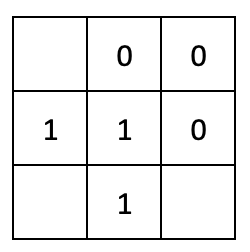
\includegraphics[width=0.8\textwidth]{hit-and-miss-kernel.png}
        \caption{Example of kernel. Cells in blank are "I don't care" valued.}
      \end{figure}
    \end{column}
  \end{columns}
\end{frame}

\begin{frame}[c]
  \frametitle{Morphological Thinning}
  \begin{block}
    {Thinnig operation}
    Given a binary image $I$ and a kernel $K$:
    \begin{equation}
      thin(I, K) = I - hit\mbox{-}or\mbox{-}miss(I, K)
    \end{equation}
    where the subtraction is the logical subtraction $X-Y = X \cap \neg Y$
  \end{block}
  \begin{itemize}
    \item A pixel $(i, j)$ is deleted (i.e. set to 0) if kernel and sub-image \textbf{do not} exacly match, otherwise is left unchanged.
    \item To obtain a skeleton of the image, $thin(I, K)$ should be repeated until no change occurs.
    \item The choice of the kernel determines which pixels are deleted from the region.
  \end{itemize}
\end{frame}

\begin{frame}
  \frametitle{Skeletonization Kernels}
  \begin{itemize}
    \item Recalling Slide~\ref{sli:skeleton} a skeleton should preserve geometric and topological characteristics of the region such as connectivity, holes, cavities etc.
    \item $thin(I, K)$ deletes pixels based on the kernel K.
    \item The two kernels below (and all their 90° rotations) allow to delete only pixels whose deletion preserves the above mentioned characteristics.
    \item In each iteration $thin(I, K)$ is executed for each of the 8 resulting kernels.
  \end{itemize}
  \begin{figure}
    \centering
    \begin{subfigure}[b]{0.45\textwidth}
      \centering
      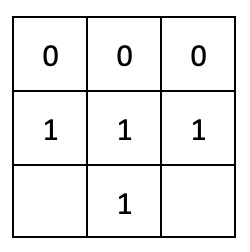
\includegraphics[width=0.6\textwidth]{border-kernel.png}
      \caption{Detects deletable border pixels.}
    \end{subfigure}
    \hfill
    \begin{subfigure}[b]{0.45\textwidth}
      \centering
      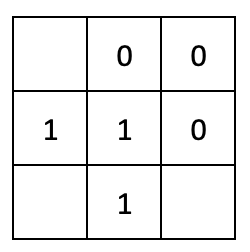
\includegraphics[width=0.6\textwidth]{corner-kernel.png}
      \caption{Detects deletable corner pixels.}
    \end{subfigure}
    \caption{Morphological thinning kernels (and all their 90° rotations)}
  \end{figure}
\end{frame}

\begin{frame}
  \frametitle{Spurs Problem}
  \begin{block}{Spurs}
    Skeletons obtained by $thin(I, K)$ with kernels presented in the previous slide can present \textbf{short spurs} produced by irregularities in the boundary of the region as shown below.
  \end{block}
  \begin{columns}
    \begin{column}{0.4\textwidth}
      \begin{figure}
        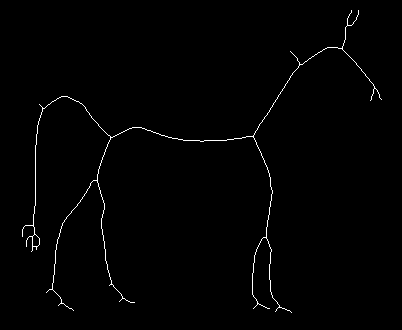
\includegraphics[width=\textwidth]{spur-example.png}
        \caption{Morphological thinning skeleton with spurs.}
      \end{figure}
    \end{column}
    \begin{column}{0.6\textwidth}
      \begin{itemize}
        \item Spurs can be removed by a process called \textbf{pruning}.
        \item Pruning is performed by applying $thin(I, K)$ with ad-hoc kernels for a \textbf{fixed amount} of iterations.
        \item Pruning until convergence would actually remove all pixels exept those which form closed loops.
      \end{itemize}
    \end{column}
  \end{columns}
\end{frame}

\begin{frame}
  \frametitle{Kernels for Spur Removal}
  By using the kernels (and all their 90° rotations) shown below is possible to remove spurs from skeleton.
  \begin{columns}
    \begin{column}{0.5\textwidth}
      \begin{figure}
        \centering
        \begin{subfigure}[b]{0.5\textwidth}
          \centering
          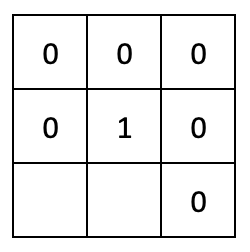
\includegraphics[width=\textwidth]{spur-1-kernel.png}
        \end{subfigure}
        \hfill
        \begin{subfigure}[b]{0.5\textwidth}
          \centering
          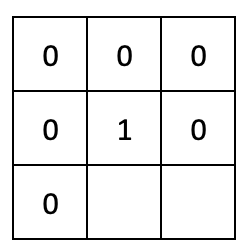
\includegraphics[width=\textwidth]{spur-2-kernel.png}
        \end{subfigure}
        \caption{Spur removal kernels}
      \end{figure}
    \end{column}
    \begin{column}{0.5\textwidth}
      After removing spurs for 10 iterations we get the following skeleton.
      \begin{figure}
        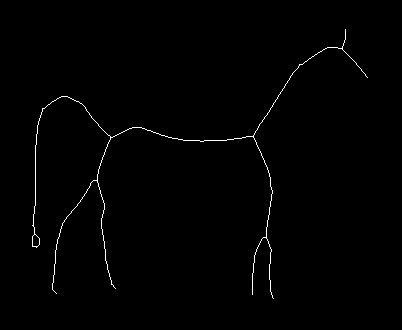
\includegraphics[width=\textwidth]{spur-removed.png}
        \caption{Skeleton after spur removal.}
      \end{figure}
    \end{column}
  \end{columns}
\end{frame}

\begin{frame}
  \frametitle{Morphological Thinning Pseudocode}
  \section{Morphological Thinning}
\begin{frame}
  \frametitle{Morphological Thinning}
  \textbf{Morphological Thinning}~\cite{morph} is a morphological operation that removes contour pixels from a region of a binary image. It relies on the \textbf{Hit-or-Miss transform} operation.
  \begin{block}
    {Hit-or-Miss transform}
    General binary morphological operation used to look for the presence of specific patterns of \emph{foreground} and \emph{background pixels} (1s or 0s respectively).
  \end{block}
  \begin{columns}
    \begin{column}{0.7\textwidth}
      \begin{itemize}
        \item Hit-or-Miss transform uses a \emph{structuring element} or \emph{kernel} to look for those patterns. \item Tipycally it is used a $3\times3$ kernel. It can contain both 1s and 0s and a special "I don't care" value.
        \item Iteration over all pixels, comparing the kernel with the underlying sub-image.
        \item \lstinline{M[i][j]}$= \begin{cases} 1 & \mbox{if } kernel =$ \lstinline{M[i-1:i+1][j-1:j+1]}$ \\ 0 & otherwise\end{cases}$
      \end{itemize}
    \end{column}
    \begin{column}{0.3\textwidth}
      \begin{figure}
        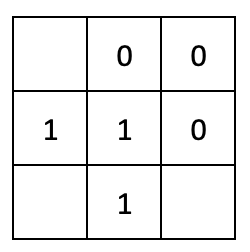
\includegraphics[width=0.8\textwidth]{hit-and-miss-kernel.png}
        \caption{Example of kernel. Cells in blank are "I don't care" valued.}
      \end{figure}
    \end{column}
  \end{columns}
\end{frame}

\begin{frame}[c]
  \frametitle{Morphological Thinning}
  \begin{block}
    {Thinnig operation}
    Given a binary image $I$ and a kernel $K$:
    \begin{equation}
      thin(I, K) = I - hit\mbox{-}or\mbox{-}miss(I, K)
    \end{equation}
    where the subtraction is the logical subtraction $X-Y = X \cap \neg Y$
  \end{block}
  \begin{itemize}
    \item A pixel $(i, j)$ is deleted (i.e. set to 0) if kernel and sub-image \textbf{do not} exacly match, otherwise is left unchanged.
    \item To obtain a skeleton of the image, $thin(I, K)$ should be repeated until no change occurs.
    \item The choice of the kernel determines which pixels are deleted from the region.
  \end{itemize}
\end{frame}

\begin{frame}
  \frametitle{Skeletonization Kernels}
  \begin{itemize}
    \item Recalling Slide~\ref{sli:skeleton} a skeleton should preserve geometric and topological characteristics of the region such as connectivity, holes, cavities etc.
    \item $thin(I, K)$ deletes pixels based on the kernel K.
    \item The two kernels below (and all their 90° rotations) allow to delete only pixels whose deletion preserves the above mentioned characteristics.
    \item In each iteration $thin(I, K)$ is executed for each of the 8 resulting kernels.
  \end{itemize}
  \begin{figure}
    \centering
    \begin{subfigure}[b]{0.45\textwidth}
      \centering
      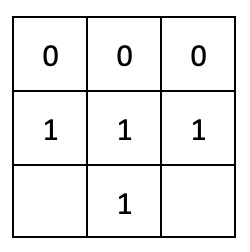
\includegraphics[width=0.6\textwidth]{border-kernel.png}
      \caption{Detects deletable border pixels.}
    \end{subfigure}
    \hfill
    \begin{subfigure}[b]{0.45\textwidth}
      \centering
      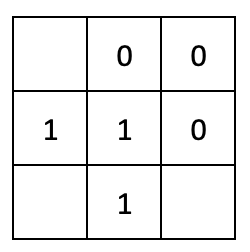
\includegraphics[width=0.6\textwidth]{corner-kernel.png}
      \caption{Detects deletable corner pixels.}
    \end{subfigure}
    \caption{Morphological thinning kernels (and all their 90° rotations)}
  \end{figure}
\end{frame}

\begin{frame}
  \frametitle{Spurs Problem}
  \begin{block}{Spurs}
    Skeletons obtained by $thin(I, K)$ with kernels presented in the previous slide can present \textbf{short spurs} produced by irregularities in the boundary of the region as shown below.
  \end{block}
  \begin{columns}
    \begin{column}{0.4\textwidth}
      \begin{figure}
        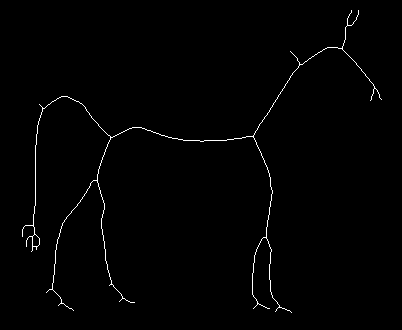
\includegraphics[width=\textwidth]{spur-example.png}
        \caption{Morphological thinning skeleton with spurs.}
      \end{figure}
    \end{column}
    \begin{column}{0.6\textwidth}
      \begin{itemize}
        \item Spurs can be removed by a process called \textbf{pruning}.
        \item Pruning is performed by applying $thin(I, K)$ with ad-hoc kernels for a \textbf{fixed amount} of iterations.
        \item Pruning until convergence would actually remove all pixels exept those which form closed loops.
      \end{itemize}
    \end{column}
  \end{columns}
\end{frame}

\begin{frame}
  \frametitle{Kernels for Spur Removal}
  By using the kernels (and all their 90° rotations) shown below is possible to remove spurs from skeleton.
  \begin{columns}
    \begin{column}{0.5\textwidth}
      \begin{figure}
        \centering
        \begin{subfigure}[b]{0.5\textwidth}
          \centering
          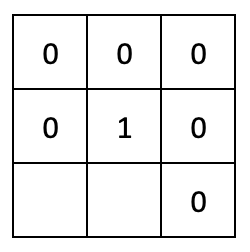
\includegraphics[width=\textwidth]{spur-1-kernel.png}
        \end{subfigure}
        \hfill
        \begin{subfigure}[b]{0.5\textwidth}
          \centering
          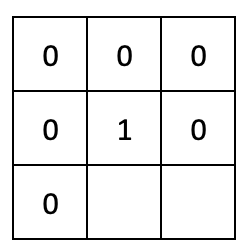
\includegraphics[width=\textwidth]{spur-2-kernel.png}
        \end{subfigure}
        \caption{Spur removal kernels}
      \end{figure}
    \end{column}
    \begin{column}{0.5\textwidth}
      After removing spurs for 10 iterations we get the following skeleton.
      \begin{figure}
        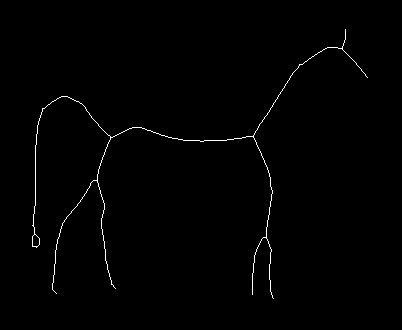
\includegraphics[width=\textwidth]{spur-removed.png}
        \caption{Skeleton after spur removal.}
      \end{figure}
    \end{column}
  \end{columns}
\end{frame}

\begin{frame}
  \frametitle{Morphological Thinning Pseudocode}
  \section{Morphological Thinning}
\begin{frame}
  \frametitle{Morphological Thinning}
  \textbf{Morphological Thinning}~\cite{morph} is a morphological operation that removes contour pixels from a region of a binary image. It relies on the \textbf{Hit-or-Miss transform} operation.
  \begin{block}
    {Hit-or-Miss transform}
    General binary morphological operation used to look for the presence of specific patterns of \emph{foreground} and \emph{background pixels} (1s or 0s respectively).
  \end{block}
  \begin{columns}
    \begin{column}{0.7\textwidth}
      \begin{itemize}
        \item Hit-or-Miss transform uses a \emph{structuring element} or \emph{kernel} to look for those patterns. \item Tipycally it is used a $3\times3$ kernel. It can contain both 1s and 0s and a special "I don't care" value.
        \item Iteration over all pixels, comparing the kernel with the underlying sub-image.
        \item \lstinline{M[i][j]}$= \begin{cases} 1 & \mbox{if } kernel =$ \lstinline{M[i-1:i+1][j-1:j+1]}$ \\ 0 & otherwise\end{cases}$
      \end{itemize}
    \end{column}
    \begin{column}{0.3\textwidth}
      \begin{figure}
        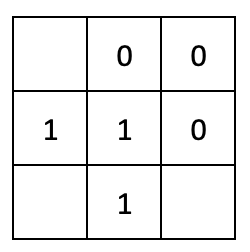
\includegraphics[width=0.8\textwidth]{hit-and-miss-kernel.png}
        \caption{Example of kernel. Cells in blank are "I don't care" valued.}
      \end{figure}
    \end{column}
  \end{columns}
\end{frame}

\begin{frame}[c]
  \frametitle{Morphological Thinning}
  \begin{block}
    {Thinnig operation}
    Given a binary image $I$ and a kernel $K$:
    \begin{equation}
      thin(I, K) = I - hit\mbox{-}or\mbox{-}miss(I, K)
    \end{equation}
    where the subtraction is the logical subtraction $X-Y = X \cap \neg Y$
  \end{block}
  \begin{itemize}
    \item A pixel $(i, j)$ is deleted (i.e. set to 0) if kernel and sub-image \textbf{do not} exacly match, otherwise is left unchanged.
    \item To obtain a skeleton of the image, $thin(I, K)$ should be repeated until no change occurs.
    \item The choice of the kernel determines which pixels are deleted from the region.
  \end{itemize}
\end{frame}

\begin{frame}
  \frametitle{Skeletonization Kernels}
  \begin{itemize}
    \item Recalling Slide~\ref{sli:skeleton} a skeleton should preserve geometric and topological characteristics of the region such as connectivity, holes, cavities etc.
    \item $thin(I, K)$ deletes pixels based on the kernel K.
    \item The two kernels below (and all their 90° rotations) allow to delete only pixels whose deletion preserves the above mentioned characteristics.
    \item In each iteration $thin(I, K)$ is executed for each of the 8 resulting kernels.
  \end{itemize}
  \begin{figure}
    \centering
    \begin{subfigure}[b]{0.45\textwidth}
      \centering
      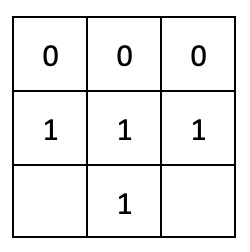
\includegraphics[width=0.6\textwidth]{border-kernel.png}
      \caption{Detects deletable border pixels.}
    \end{subfigure}
    \hfill
    \begin{subfigure}[b]{0.45\textwidth}
      \centering
      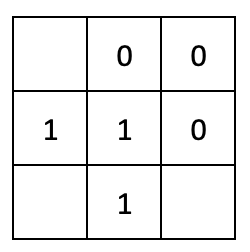
\includegraphics[width=0.6\textwidth]{corner-kernel.png}
      \caption{Detects deletable corner pixels.}
    \end{subfigure}
    \caption{Morphological thinning kernels (and all their 90° rotations)}
  \end{figure}
\end{frame}

\begin{frame}
  \frametitle{Spurs Problem}
  \begin{block}{Spurs}
    Skeletons obtained by $thin(I, K)$ with kernels presented in the previous slide can present \textbf{short spurs} produced by irregularities in the boundary of the region as shown below.
  \end{block}
  \begin{columns}
    \begin{column}{0.4\textwidth}
      \begin{figure}
        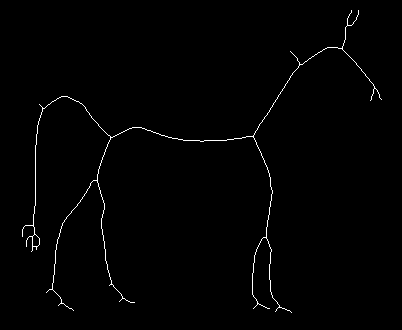
\includegraphics[width=\textwidth]{spur-example.png}
        \caption{Morphological thinning skeleton with spurs.}
      \end{figure}
    \end{column}
    \begin{column}{0.6\textwidth}
      \begin{itemize}
        \item Spurs can be removed by a process called \textbf{pruning}.
        \item Pruning is performed by applying $thin(I, K)$ with ad-hoc kernels for a \textbf{fixed amount} of iterations.
        \item Pruning until convergence would actually remove all pixels exept those which form closed loops.
      \end{itemize}
    \end{column}
  \end{columns}
\end{frame}

\begin{frame}
  \frametitle{Kernels for Spur Removal}
  By using the kernels (and all their 90° rotations) shown below is possible to remove spurs from skeleton.
  \begin{columns}
    \begin{column}{0.5\textwidth}
      \begin{figure}
        \centering
        \begin{subfigure}[b]{0.5\textwidth}
          \centering
          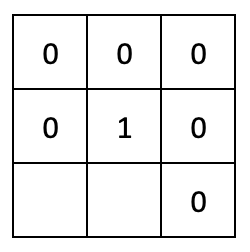
\includegraphics[width=\textwidth]{spur-1-kernel.png}
        \end{subfigure}
        \hfill
        \begin{subfigure}[b]{0.5\textwidth}
          \centering
          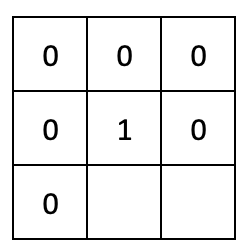
\includegraphics[width=\textwidth]{spur-2-kernel.png}
        \end{subfigure}
        \caption{Spur removal kernels}
      \end{figure}
    \end{column}
    \begin{column}{0.5\textwidth}
      After removing spurs for 10 iterations we get the following skeleton.
      \begin{figure}
        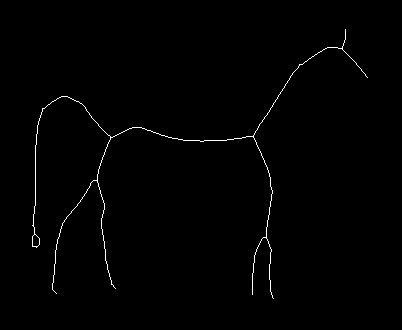
\includegraphics[width=\textwidth]{spur-removed.png}
        \caption{Skeleton after spur removal.}
      \end{figure}
    \end{column}
  \end{columns}
\end{frame}

\begin{frame}
  \frametitle{Morphological Thinning Pseudocode}
  \input{assets/pseudocode/morph.tex}
\end{frame}

\end{frame}

\end{frame}

\section{Lee's 3D Skeletonization}
\section{Wrap-up}
\begin{frame}
  \frametitle{Bibliography}
  \printbibliography
\end{frame}
\begin{frame}
  \frametitle{Conclusion}
  \begin{center}
    \Huge Thank you for your attention.
  \end{center}
\end{frame}

\end{document}
